\documentclass[12pt] {report}

\usepackage[dvipsnames]{xcolor}
\usepackage[utf8]{inputenc}
\usepackage [top=3cm, bottom=3cm, left=35mm, right=25mm] {geometry}

% Font style:
\usepackage{fontspec}
\setromanfont[
BoldFont=GARABD.ttf,
ItalicFont=GARAIT.ttf,
BoldItalicFont=GARA.ttf,
]{GARA.ttf}

\setsansfont[
BoldFont=GARABD.ttf,
ItalicFont=GARAIT.ttf,
BoldItalicFont=GARA.ttf,
]{GARA.ttf}

\setmonofont[Scale=1,
BoldFont=GARABD.ttf,
ItalicFont=GARAIT.ttf,
BoldItalicFont=GARA.ttf,
]{GARA.ttf}

\usepackage{pdfpages}


\usepackage[natbibapa]{apacite}

\usepackage{multirow}
\usepackage{array}
\usepackage{longtable}

\usepackage{graphicx}




\usepackage{graphicx} %package to manage images
\graphicspath{ {./images/} }
\usepackage[rightcaption]{sidecap}
\usepackage{wrapfig}


\usepackage{caption}
\usepackage{subcaption}

\usepackage{amsmath}

\usepackage{lscape}


\usepackage[utf8]{inputenc}
\usepackage[english]{babel}


\usepackage{chngcntr}   
\counterwithin{equation}{chapter}



\usepackage[labelfont=bf]{caption}
\captionsetup{labelfont=bf}

%\usepackage[demo]{graphicx}

\usepackage{hyperref}

\usepackage{indentfirst}

\title{Clustering three-way data structures: \protect \linebreak a time series approach}
\author{Marta Dainovich}
\date{\today}

\DeclareMathOperator*{\argmax}{arg\,max}
\DeclareMathOperator*{\argmin}{arg\,min}


%%%%%%%%%%%%%%%%%%%%%% BEGIN DOC %%%%%%%%%%%%%%%%%

\pagenumbering{roman}

\begin{document}

\date{}
\begin{titlepage}
\begin{center}

\begin{figure}[ht!]
    \centering
    
\includegraphics[scale=0.5]{images/FEP.PNG}
\end{figure}

\vspace*{0.7in}
{\LARGE \textbf{ {\scshape NAME OF THE PROJECT}}}
\par
\vspace{0.4in}
{\large By}
\par
\vspace{0.4in}
{\large AUTOR}
\par
\vspace{1in}
{\large Master Thesis in Moodeling, Data Analysis \protect \linebreak and Decision Support Systems}
\par
\vspace{0.8in}
\end{center}
{\large Supervised by:} \\ 
\par
{\large Professor X}
\par
\vspace{0.10in}
{\large Professor Y}
\vspace{1in}
\begin{center}
{\large \textbf{Faculdade de Economia}}
\par
\vspace{0.10in}
{\large Universidade do Porto}
\par
\vspace{0.2in}
{\large 2019}
\end{center}
\end{titlepage}


\thispagestyle{empty}

\newpage

\chapter*{Biographical note}



\addcontentsline{toc}{section}{Biographical note}
\setcounter{page}{2}

\newpage

\chapter*{Acknowledgements}








\addcontentsline{toc}{section}{Acknowledgements}
\setcounter{page}{3}



\newpage

\chapter*{Abstract}
This work aims to relate the press conferences of the European central bank, for a period defined later, with the macroeconomic scenario and with real European macroeconomic variables. As exposed by Shapiro (2019a, 2019b, 2020) it is possible to better understand what happens in the real economy from minutes and reports from central banks, allowing a correlation with different macroeconomic scenarios. The methodology used encompasses natural language processing techniques, in terms of tokenization. The tested relationships take into account endogeneities in the macroeconomic scenario and an autoregressive vector is defined in order to correct the problem. Finally, impulse response functions will be used for model simulations that corroborate the approach used.

\par
\vspace{0.5in}    
    
\noindent
{\bf Keywords:} Sentiment analysis, Central bank, Text mining, Vector Autoregressive



  
\addcontentsline{toc}{section}{Abstract}
\setcounter{page}{4}


\newpage
\chapter*{Resumo}




\par
\vspace{0.5in}

\noindent
{\bf Palavras-chave:} palavra1, palavra2....
\addcontentsline{toc}{section}{Resumo}
\setcounter{page}{5}


%Contents:
\newpage
\tableofcontents

\newpage
\listoffigures

\newpage 
\listoftables

\newpage
\pagenumbering{arabic}
\chapter{\textbf{Introduction}}  \label{introduction}
\pagenumbering{arabic}

Economics decisions, in particular monetary policies, are based in resolutions provided by central banks. However, these resolutions are not always clear, especially for layman. Central banks minutes contain, for instance, much more information than it seems, particularly if a set of texts are considered for a conjunctural or structural analysis.\\

On occasion, the comprehension of a set of texts could be complex enough for a human to perform: the analysis may be referring to thousands or even millions of pages, depending on the purpose of the understanding. Nevertheless, problems like these are increasingly likely to be resolved due to advances in computational fields. Technics and tools such as Natural Language Processing (NLP) and text mining are being strongly used for a better comprehension and understanding of what a text, or a set of text (corpus), actually means or expresses.\\

Nowadays it is possible to recognize patterns on search pages as Google and Yahoo utilising text analysis in order to predict macroeconomics variables or even increase understanding of consumer behaviour. In recent research, Bholat, Hansen, Santos, \& Schonhardt-Bailey (2015) consider that even though the advances that have taken place in the field of computing are significant, the applicability of text mining in economics is still not used the way it could be.\\

An alternative approach of application still in the field of NLP is the sentiment analysis. Basically, it is “the task of identifying positive and negative opinions, emotions, and evaluations” (Wilson, Wiebe, \& Hoffmann, 2005, p.1). Sentiment analysis allows to extract information that usually a human being could not do, due to the amount of text, or even the difficulty to recognizing unstructured patterns.\\	

Another paper written by Nyman, Kapadia, \& Tuckett (2021) considered the possibility of a sentiment index, based in social media, for measure of excitement or anxiety about the financial conjunctural situation. The index would work as a proxy for the market sentiment: bullish or bearish. The ratio of the index would be, then, compared with historical events and others financial indicators (Nyman et al. 2021).\\

Gradually, technics and tools such as sentiment analysis and text mining has been used with implementations in the economic field. It is not hard to find correlations between macroeconomic variables and sentiment analysis extracted from media (Ostapenko, 2020) or even parliament hearings from central banks (Fraccaroli \& Giovannini, 2020).\\

This work has as its main objective the analysis and investigation of how textual patterns provided by the ECB can indicate and correlate with conjunctural and structural moments in the economy (especially in macroeconomics). From structured data taken from press conferences of the European central bank and monetary policy resolutions, understand how “words” and “expressions” can indicate a period of recession, or even verify the credibility of the central bank from its “expressions”. NLP techniques have been increasingly used in order to capture patterns practically imperceptible to the human eye, the use of this technique in the economic field could be of great advancement and usefulness for a better understanding of what central banks are really indicating (through textual documents), and not only reduce the indication of the central bank based on its own resolutions.\\

The greatest relevance and contribution of this work is the use of ECB press conferences as an indicator of sentiments - not as done before, where the main references came from monetary policy reports or speeches. Starting from this point, it will be possible to compare the results obtained with previous works so that an “asymptotic” relationship in terms of results is expected.\\

This final report is fundamentally divided according to the division of the final dissertation, with the exception of the parts referring to the final results and conclusion. Section 2 addresses the literature review, fundamentally alluding to text mining, sentiment analysis, and econometric applications; section 3 deals with the methodology used in the work, reviewing concepts of more computational approaches such as web scraping and NLP techniques; section 4 focuses on the division of the work plan as well as a provisional index of the dissertation; section 5 presents the textual references of this work.



\chapter{\textbf{Literature review}}  \label{chapter:lit}

According to Chowdhury, (2003) “Natural Language Processing (NLP) is an area of research and application that explores how computers can be used to understand and manipulate natural language text or speech to do useful things. NLP researchers aim to gather knowledge on how human beings understand and use language so that appropriate tools and techniques can be developed to make computer systems understand and manipulate natural languages to perform desired tasks” (Chowdhury, 2003, p.1).\\

One of the advantages of utilising documents, texts, and minutes, is the possibility of working with quantitative and qualitative data at same time (Bholat et al., 2015, p.1). Working with both types of data it is possible to carry out studies and statistical inferences that would not be possible with just structured data – even though the applicability of these type of study is vast, it has only been used in economics for a short time.\\

Recently, Shapiro, Sudhof \& Wilson (2020) reported that an economic index, created by the authors, based on sentiment analysis from economic papers was related with macroeconomic variables. For this paper the authors consider real variables as real interest rate, inflation, domestic consumption, and real growth domestic product for the American economy. They evaluated whether the index score would be related to the behaviour of these variables.

\begin{figure}[!h]
    \centering
    \caption{Impulse response of a positive news sentiment shock on economic activity}
    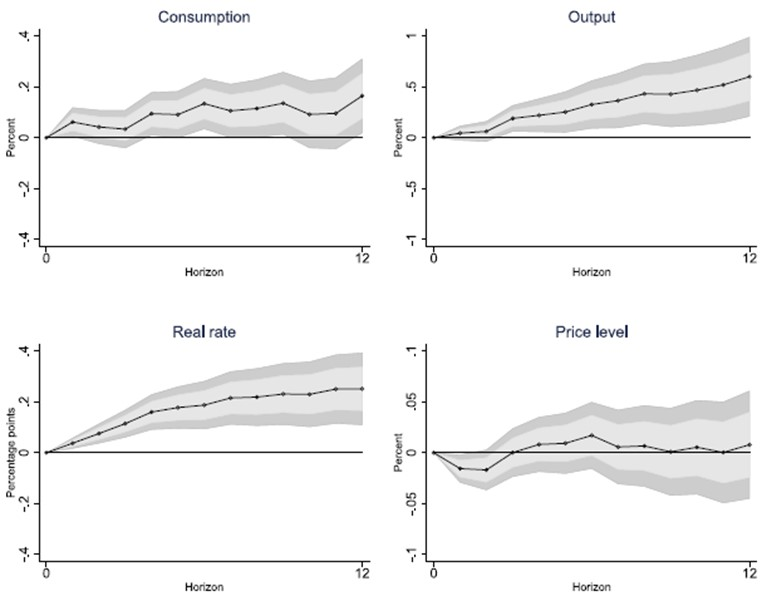
\includegraphics[width=.8\textwidth]{images/image1.jpg}
    \caption*{Source: \cite[p.16]{shapiro2020measuring}}
    \label{fig:my_label}
\end{figure}

Utilising statistical and econometrics technics, specifically the Vector Autoregressive (Sims, 1980), the authors showed by the impulse response function that it is possible to understand what happens to the economy when considering the score of the index: given a positive shock at the index sentiment score, it affects positively the consumption, the interest rate, and the output. The effect at the price level, however, is transitory while the persistence of the shock at the other variables gradually gets higher: “Extending the horizon out further […] indicates that the responses of consumption, output, and the real rate peak between 12 and 18 months after the shock before gradually waning” \citet[p.16]{shapiro2020measuring}.\\
\cite
Another study tried to estimate the central bank objectives using text analysis \cite{shapiro2021taking}. This time the authors sought to understand the main objective of a central bank (Federal Reserve Board) utilising its internal discussions (U.S. Federal Open Market Committee’s - FOMC). They implemented a model with the aim of incorporating text analysis in structural estimations in order to take into account the “weights” of the central banker’s preferences. An index of negativity was created based on a dictionary \cite{loughran2011liability} of economic terms in order to implement a new approach to estimate the parameters of a central bank objective function: for each hearing of the FOMC was created a score based in the frequency of positive and negative word of the hearing. The result presented by the authors is that usually the models do not consider those preferences, thus the incorporation of such technics would significantly improve the models and its interpretations, helping to explain what is, in fact, the objective function of a central bank.\\

In order to complement the literature of sentiment analysis in economics, \cite{ostapenko2020macroeconomic} contributed analysing “how the change of tone or topic in newspaper affects the macroeconomy”. The author transformed articles from newspaper (employing a topic model and vector representation of documents with clustering) into time series and based on this time series, evaluated the sentiment of each article. On occasion, the article demonstrated that given a new shock in the sentiment of the articles, it could mean an increase over the long run, in output and consumption – it also affects the inflation and interest rate, however transiently.\\

Progressively, text mining, sentiment analysis and other techniques end up helping the field of economics to understand better what is happening and what is the relation of the conjunctural or structural scenarios with social expressions. Sentiment analysis helps to understand the consumption behaviour, or even how the media can influence or even chance an economic scenario. Text mining allows to extract qualitative and quantitative information from a text or a corpus. Sooner or later NLP will be increasingly used for a better understanding of the world or the field of economic science.\\

Overall, the approach of researchers and contributors in this area is particularly similar. In terms of estimations, there is a consensus on the importance of treating endogeneity related to macroeconomic relations: when a model is estimated, the use of an autoregressive vector is generally chosen, even if based on an unorthodox approach in the statistical field, considering from methods of Bayesian estimations to autoregressive vector with signal constraints \citet{santos2020indice}.\\

In terms of descriptive analysis, or in terms of classifiers, the approach varies according to the chosen methodology, generally with greater emphasis on classification techniques such as support vector machine, k-means neighbours, or k-nearest neighbour (KNN) \citet{ostapenko2020macroeconomic}. Still, it is worth noting that approaches that assume NLP techniques such as tokenization (see section 3) are still little used, especially with regard to estimations: it is important to emphasize that not using techniques such as tokenization in estimations can create a lack of results in terms of contribution to economic science, given the fact that a better understanding of what happens in the economic scenario is possible and plausible based on a better understanding of how terms and expressions are related to economic cycles.\\





%\newpage
\chapter{\textbf{Methodology}} \label{cap:methodology}

%As stated before, as this is a quantitative and somewhat qualitative analysis, some specific techniques will have to be used.\\

%First, when it comes to an analysis that takes into account the way in which the European Central Bank expresses itself. Thus, it is necessary that the work takes shape around either ECB speeches\footnote{\url{https://www.ecb.europa.eu/press/key/date/html/index.en.html}} or press conferences \footnote{\url{https://www.ecb.europa.eu/press/pr/date/html/index.en.html}}. Regarding the first, this becomes easier, given the fact that the ECB releases the speeches dataset. In relation to the second one, a more robust work is needed.

%\section{Data} \label{sec:data}

%Given that the format in which press conferences are found on the European central bank website is unstructured (texts are not organized in a database, for example), a more alternative approach to obtaining textual data is needed. Web scraping is the alternative that allows to obtain these data in a computational way, without having to do the gruelling work of locating link by link, copying the text, storing, and organizing it.\\

%The basic principle of web scraping is to locate specific tags in HTML that make it possible to locate and obtain data, through an algorithm that instructs the computer to do this. After obtaining the tags and texts, the selected texts (or web pages) are stored in a dataset and organize the data. This technique would be used to obtain ECB press conferences. After the organization of the database, natural language processes are used for the analysis of textual documents.\\

%The other basic required time series (relating to macroeconomic variables) are available on the FRED website and are real output growth, output gap, unemployment, natural unemployment, inflation (consumer price index), and consumer confidence\footnote{The variables “natural unemployment” and “output gap” for being unobservable would be obtained from the Hodrick-Prescott filter}.

%\section{Tokenization} \label{sec:tokenization}

%Tokenization is basically the division of a sentence, sentence, paragraph, or an entire text document into smaller units, such as individual words or even terms. Each of these smaller units is called tokens.\\

%From tokenization it is possible to count specific words, specific textual expressions and analyse how variations of words and expressions can indicate specific and relevant periods in terms of conjecture or economic structure. For example, given the term “inflation target”, from tokenization it is possible to visualize the appearance of this term in ECB press conferences - it would be plausible to question whether the appearance of certain terms appear more in times of recessions or expansions of the economic cycle.\\

\section{Sentiment Lexicons} \label{sec:lexicons}

\subsection{Polarity-based Lexicons} \label{subsec:polbas}
\subsection{Valence-based Lexicons}

%In the scope of sentiment analysis, 

%In the scope of sentiment analysis, it is necessary to use a dictionary of sentiments to detect polarities of sentiments and positive/negative scores. From the scores and polarities, it is possible to obtain a sentiment index that generates a possible correlation with the macroeconomic scenario. Basically, a sentiment dictionary works by indicating a specific punctuation for each word, taking into account punctuation and connectives. That is, depending on how a sentence or sentence is written, its polarity (score) varies.

\subsection{VADER – Valence Aware Dictionary for sEntiment Reasoning} \label{subsec:vader}

VADER, or Valence Aware Dictionary for sEntiment Reasoning is a lexicon initially created as a parsimonious lexicon for social media text. However, it has been used in general cases of textual sentiment analysis given it's benchmarks compared to other lexicons or even machine learning oriented techniques ``relying on Naive Bayes, Maximum Entropy, and Support Vector Machine (SVM) algorithms'' \citep[p.216]{hutto2014vader}. Differently of most part of lexicons, VADER was created taking into account a combination of qualitative and quantitative methods to empirically validates and produces a \textit{golden-standard} sentiment lexicon \cite{hutto2014vader}.\\

Due to the fact that VADER is an open-source lexicon, it is relatively simple to modify -- even if it is not what was done in this work, it would be possible, if necessary, merging VADER with some other lexicons, with the objective of creating a more complex and dense lexicon focused on economic science and finance. This lexicon has about 7520 words and textual forms with a classified score compound which after normalized varies from -1 to 1 such that:
\begin{align} \label{eq:vaadercoumpond}
    score_ = \begin{cases}
                positive\quad if \quad compound > 0.05\\
                neutral\quad if \quad 0.05 \geq compound \geq -0.05\\
                negative\quad if \quad compound < 0.05
              \end{cases} \qquad \forall\quad compound \in (-1, 1)
\end{align}

The positive, neutral and negative scores are ratios for each category that the text or expression fells on: 
\begin{quote}
    ``These are the most useful metrics if you want to analyze the context \& presentation of how sentiment is conveyed or embedded in rhetoric for a given sentence. For example, different writing styles may embed strongly positive or negative sentiment within varying proportions of neutral text -- i.e., some writing styles may reflect a penchant for strongly flavored rhetoric, whereas other styles may use a great deal of neutral text while still conveying a similar overall (compound) sentiment. As another example: researchers analyzing information presentation in journalistic or editorical news might desire to establish whether the proportions of text (associated with a topic or named entity, for example) are balanced with similar amounts of positively and negatively framed text versus being "biased" towards one polarity or the other for the topic/entity'' \cite{vadergit}.
\end{quote}

Even when VADER excels when in social media, it's scores benchmarks when considered newspaper editorials are higher above the other lexicons or machine learning techniques (Table \ref{tab:vaderscore}) -- ``Surprisingly, when we further inspect the classification accuracy, we see that VADER (F1 = 0.96) actually even outperforms individual human raters (F1 = 0.84) at correctly classifying the sentiment of tweets into positive, neutral, or negative classes'' \citep[p.216]{hutto2014vader}.

\begin{table}[!h]
\centering
\caption{VADER 3-class classification performance as compared to individual human raters and 7 established lexicon baselines}
\begin{tabular}{l|c|c|c|c}
\hline
\multicolumn{2}{l|}{Correlation to ground truth} & \multicolumn{3}{l}{Classification Accuracy Metrics}   \\ \cline{3-5} 
\multicolumn{2}{l|}{(mean of 20 humans raters)}  & Overall Precision & Overall Recall & Overall F1 score \\ \hline
\multicolumn{5}{c}{NY Times Editorials (5,190 article snippets)}                                         \\ \hline
Ind. Humans                & 0.745               & 0.87              & 0.55           & 0.65             \\
VADER                      & 0.492               & 0.69              & 0.49           & 0.55             \\
Hu-Liu04                   & 0.487               & 0.70              & 0.45           & 0.52             \\
SCN                        & 0.252               & 0.62              & 0.47           & 0.38             \\
GI                         & 0.362               & 0.65              & 0.44           & 0.49             \\
SWN                        & 0.262               & 0.57              & 0.49           & 0.52             \\
LIWC                       & 0.220               & 0.66              & 0.17           & 0.21             \\
ANEW                       & 0.202               & 0.59              & 0.32           & 0.35             \\
WSD                        & 0.218               & 0.55              & 0.45           & 0.47             \\ \hline 
\end{tabular}
\caption*{Source: \citep[p. 223]{hutto2014vader}}
\label{tab:vaderscore}
\end{table}



%One of the most used dictionaries today for detecting sentiments is the Valence Aware Dictionary for Sentiment Reasoning (VADER). The choice of VADER as the main dictionary is due to some facts: “it is bigger, yet just as simply inspected, understood, quickly applied (without a need for extensive learning/training) and easily extended” (Hutto \& Gilbert, 2014. p.1).\\

%Due to the fact that VADER is an open-source dictionary, it is relatively simple to modify the dictionary so that it has a greater focus on the economic part. The change needed is likely to be fundamentally within the word scores: that is, inserting specific words like “price” or “prices” into the dictionary scope and assigning a referent score based on other economics-based sentiment dictionaries. As well as, if necessary, merging VADER with some other dictionary with a more economical approach.\\

%Once you have the scores for the texts as well as the tokens, it becomes possible to relate the variation of certain economic words/terms with the variation in the sentiment of the corpus or of each press conference. The next step is, then, to relate the obtained index (either polarity or the score itself) with macroeconomic variables.\\

\subsection{Loughran-McDonald: LM-SA-2020}  \label{subsec:loughran}

The other lexicon used in this work is the LM-SA-2020 and was the same provided by \cite{loughran2011liability}. Fundamentally, the difference between this one is the composition: the authors developed a dictionary with the purpose of revising the traditional lexicons in which certain words are or are not considered positive or negative in the economic and financial sphere \citep[p. 35]{loughran2011liability}:

\begin{quote}
    ``The motivation for building the LM-SA-2020 word list was based on an experiment using the above-mentioned original lists to detect sentiment-carrying words in South African financial article headlines''\citep[p. 1]{lmdata}
\end{quote}

This lexicon uses 808 financial articles and only about 37\% of the headlines actually corresponded to the expected sentiments (either in terms of words or expressions) given the articles verified by the authors\citep{loughran2011liability}. In terms of benchmark, with adding economic words and removing others in terms of polarity, sentiment detection and prediction increased by about 29\% when added to NLTK's WordNet\footnote{\url{https://www.nltk.org/howto/wordnet.html}}.\\

The results obtained by the authors were based on an analysis of two samples of reference articles: first, the authors considered a sample of 10 thousand files related to firms subject to shareholder litigation under Rule 10b-5. The other sample used by the authors considers \cite{doyle2007accruals}, between August 2002 and November 2005, companies disclosed at least one material deficiency in internal control \citep[p. 41]{loughran2011liability}. The authors estimated different models\footnote{In fact, 28 different Logit models were estimated. The economic variables used were The number of shares outstanding times the price of the stock as reported by CRSP on the day before the file date; Book-to-market (Derived from the Compustat and CRSP data items as specified in Fama and French (2001). The variable is based on the most recent Compustat data no more than 1 year before the file date. After eliminating observations with negative book-to-market, we winsorize the book-to-market variable at the 1\% level); The volume of shares traded in days [−252, −6] prior to the file date divided by shares outstanding on the file date. At least 60 observations of daily volume must be available to be included in the sample; The prefile date Fama–French alpha based on a regression of their three-factor model using days [−252, −6]. At least 60 observations of daily returns must be available to be included in the sample; The percent of institutional ownership reported in the CDA/Spectrum database for the most recent quarter before the file date. The variable is considered missing for negative values and winsorized to 100\% on the positive side; The average volume of the 4-day event window [0, 3], where volume is standardized based on its mean and standard deviation from days [−65, −6]; The root-mean square error from a Fama–French three-factor model for days [6, 252], with a minimum of 60 daily observations; Standardized unexpected earnings for the quarterly earnings announced within 90 days after the 10-K file date. The actual earnings and the analyst forecast consensus (mean) are from I/B/E/S unadjusted files, which are used to avoid the rounding issue. The unexpected earnings are standardized with stock price; The standard deviation of analysts’ forecasts in the most recent period prior to the earnings announcement used to calculate SUE, scaled by the stock price at the end of the quarter; The monthly change in the mean of analysts’ forecasts, scaled by the stock price in the prior month; and a dummy variable set equal to one for firms whose shares are listed on the NASDAQ stock exchange, else zero\citep[p.63]{loughran2011liability}} to reach the final conclusion that the lexicon accuracy increases with the addition or change of economic terms.\\

The lexicon created by the authors also allows for a more comprehensive classification in which, in addition to classifying certain words and terms as positive and negative, it also classifies them as ``uncertainty, litigious, strong modal, and weak modal words''\citep[p.62]{loughran2011liability}: 
\begin{quote}
    ``The paper finds evidence that some word lists are related to market reactions around the 10-K filing date, trading volume, unexpected earnings, and subsequent stock return volatility. [\dots] we show that financial researchers should be cautious when relying on word classification schemes derived outside the domain of business usage. Applying nonbusiness word lists to accounting and finance topics can lead to a high misclassification rate and spurious correlations''\citep[p.62]{loughran2011liability}
\end{quote}





%\section{Vector Autoregressive} \label{sec:var}




%\newpage
\chapter{\textbf{European Central Bank Documents: A Case Study}}

Given the need to corroborate and expand research in the area of sentiment analysis applied to the economic sciences -- and based on the examples already observed in chapter \ref{chapter:lit}, an application in a case study is proposed here.\\



\section{Problem and Data Description}



\section{Experimental Setup}
% cross validation

\section{Modeling}
%pre-processing
%learning algorithms
%evaluation metrics
\section{Experimental Results}

\section{Discussion}


%\newpage
\chapter{Conclusions}  \label{chapfinal}




\newpage
\bibliographystyle{apacite}
\bibliography{References.bib}

\newpage 

\chapter*{Appendix}
\addcontentsline{toc}{chapter}{Appendix}
\renewcommand*{\thesection}{\Alph{section}}
\pagenumbering{roman}
\newpagew


% Appendix 1
\section{List of Z.} 



\newpage



% Appendix 2
\newpage

\section{Description X.}








\end{document}



